\chapter{Grammatik im Lehramtsstudium}
\label{sec:grammatikimlehramtsstudium}


\section{Grammatik in der Schule}
\label{sec:grammatikinderschule}

Die Frage nach der Rolle von Grammatik im Lehramtsstudium kann nicht losgelöst von der Rolle der Grammatik im Schulunterricht diskutiert werden.
In diesem Abschnitt wird daher bündig ein Konzept von Grammatik in der Schule diskutiert.



\section{Grammatik im Lehramtsstudium}
\label{sec:grammatikimlehramtsstudium}



\section{Kenntnisse, Erwartungen und Motivationen von Studierenden}
\label{sec:kenntnisseerwartungenundmotivationvonstudierenden}

\subsection{Grammatikkenntnisse von Studierenden}
\label{sec:grammatikkentnissevonstudierenden}

In \citet{SchaeferSayatz2017a} berichten Ulrike Sayatz und ich ein Experiment (im wissenschaftlichen Sinn des Worts), mit dem wir den letzten Punkt des vorangehenden Abschnitts untersucht haben.
Konkret haben wir evaluiert, welche schulgrammatischen Kenntnisse Studierende am Anfang des Studiums haben.
Es ging uns also um die berüchtigten \textit{schulischen Vorkenntnisse}.

Für unsere Studie gab es verschiedene Vorläufer.
Besonders medienwirksam wurden 2007 die Ergebnisse von einer Art Studieneingangstest berichtet, der in Bayern durchgeführt wurde und laut der journalistischen Aufbereitung \citep{Spiegelonline2007,Szonline2007} ergab, dass Studierende der Germanistik nicht ausreichend durch die Schule auf das Studium vorbereitet würden.
Nach einer Umrechnung der Ergebnisse in Noten wäre über die Hälfte der Teilnehmenden durchgefallen.
Die betroffenen Studierenden dürften sich allerdings durch die Art der Formulierungen, mit denen in der Presse operiert wurde, lediglich gedemütigt und keinesfalls motiviert fühlen.
Spiegel Online spricht von einem "`Grammatik-Fiasko"', bei dem Studierende "`mit Karacho durchgefallen"' seien.
Noch weiter treibt es die Süddeutsche Zeitung Online, die im genannten Artikel ausführt, die "`Germanistik-Studenten"' hätten sich "`blamiert"', und viele von ihnen seien "`Grammatik-Nieten"'.
Die Unterschiede in der konkreten Wortwahl zeigen, dass es sich hier um eine zwar gleichermaßen reißerische, aber dennoch voneinander unabhängige journalistische Aufbereitung handelt, nicht etwas um wörtliche Zitate der Durchführenden des Tests.
Trotzdem schreibt die Presse weiter, die "`Professoren [seien] erschüttert"' (Spiegel Online), und es müsse folglich "`in der Schule wieder mehr Grammatik gepaukt"' werden (Süddeutsche Zeitung Online). 
Einen größeren Schaden an der Sache können Medienberichte kaum auslösen.
In der Presse werden vor allem die Studierenden geradezu als die Schuldigen aufgebaut und entsprechend als blamable Nieten usw.\ tituliert.
Für die intendierte Sache, also eine Stärkung des Grammatikunterrichts an Schulen, leistet dies in jedem Fall keinen Beitrag.
Höchstens lehnt sich das angepeilte Zeitungspublikum zufrieden in der Gewissheit zurück, dass eben die Schule und die Jugend heutzutage nichts mehr taugen.%
\footnote{Ich wiederhole, dass ich mich hier auf die journalistische Aufarbeitung beziehe.
Diese Formulierungen stammen gewiss nicht von den Durchführenden der Studie.}

Unabhängig von der journalistischen Verarbeitung gibt es aber ein weiteres Problem mit solchen Tests.
Das Ziel der Durchführenden in Bayern war es wohl, den Grammatikunterricht an Schulen zu stärken, indem entsprechende Wissenslücken aufgezeigt wurden.
Das Argument scheint dabei gewesen zu sein, dass Studierende nach ihrer Schulzeit nicht hinreichend auf das Germanistikstudium vorbereitet seien.
Das ist allerdings, wie weiter unten in diesem Kapitel argumentiert wird, überhaupt nicht das Ziel des schulischen Unterrichts in der Grammatik des Deutschen, ebensowenig wie es das Ziel des Geschichtsunterrichts ist, auf ein Studium der Geschichtswissenschaft vorzubereiten.
Noch viel weniger ist das Ziel des Deutschunterrichts das "`Pauken von Grammatik"'.
Sowohl die Fachdidaktik des Deutschen als auch die didaktisch informierte germanistische Sprachwissenschaft wird selbstverständlich einen Nürnberger Trichter für deklaratives schulisches Grammatikwissen als Absurdität zurückweisen.

Neben diesem Versuch eines Eingangstests gibt es eine aktuelle aktive Diskussion um Funktionen und Nutzen von Studieneingangstests (siehe vor allem \citealt{Schindler2016}, aber \zB auch \citealt{Bremerichvos2016} und \citealt{FuhrhopTeuber2016}).
\citet[16]{Schindler2016} benennt neben der Funktion im Sinne einer Zulassungsschranke für das Studium vor allem zwei Funktionen solcher Tests, nämlich erstens die Diagnostik für das studierende Individuum, anhand derer gezielt Defizite erkannt und rechtzeitig ausgeglichen werden können.
Zweitens führt die Autorin an, dass Eingangstests Bewusstsein und Interesse für die Inhalte des Fachs bei Studierenden wecken können.
In \citet[226]{SchaeferSayatz2017a} argumentieren wir, dass eine weitere Funktion der Tests die Optimierung der Lehre im Studium im Sinne einer Ausrichtung auf die Bedürfnisse der Studierenden sein sollte.
Hier werden jetzt die wesentlichen Ergebnisse des Experiments berichtet, vor um bei Studierenden das Bewusstsein für die Inhalte des Fachs und die Verbindung zwischen Schulgrammatik und linguistischem Fachwissens zu wecken (Schindlers zweite Funktion), und um Lehrende anzuregen, ähnliche Evaluationen vorzunehmen und ihre Lehrinhalte und Lehrmethoden entsprechend an die Ergebnisse anzupassen (die von \citealt{SchaeferSayatz2017a} benannte Funktion).

Wir haben 220 Studierende der Freien Universität Berlin, die überwiegend in Berlin und Brandenburg zur Schule gegangen sind, einen freiwilligen anonymen Test vorgelegt, der aus gezielt ausgewählten Aufgaben aus Lehrwerken bestand, die in diesen Bundesländern für die Jahrgangsstufen sechs bis zehn (in einem Fall für die Grundschule) zugelassen sind.
Es handelte sich also um Aufgaben, die die Studierenden so oder ähnlich wahrscheinlich in ihrer Schulzeit gelöst haben.
Insgesamt wurden zehn Aufgaben ausgewählt und ausgewertet, die verschiedene Schwierigkeitsgrade und verschiedene Themen der Grammatik abdeckten, die auf der Seite der systemexternen Funktion ebenfalls verschiedenen Bereichen zuzuordnen sind.
Die Teilnehmenden, die aus allen Semestern des BA-Studiums kamen, studierten zu 37,7\% Grundschullehramt (83 Personen), zu 37,3\% Deutsch für das Lehramt (82 Personen), zu 23,2\% Deutsch als Fachwissenschaft (51 Personen) und zu 1,8\% andere Fächer (4 Personen).
Zunächst wurde überprüft, ob wirklich durchweg ungenügende "`Leistung"' erbracht wurde.
Abbildung~\ref{fig:grammatikkentnissevonstudierenden001} zeigt, dass dies nicht der Fall ist.

\begin{figure}[htpb]
  \centering
  \resizebox{0.9\textwidth}{!}{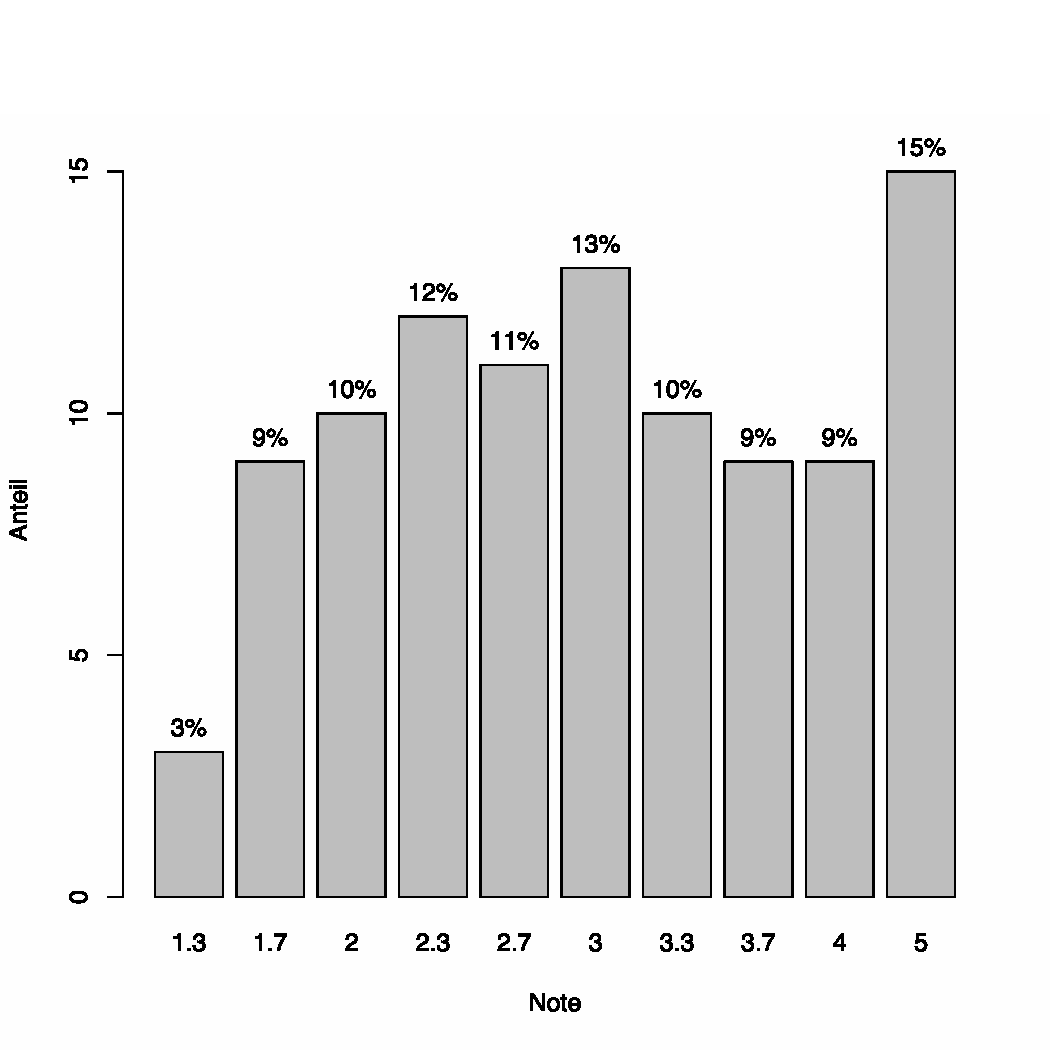
\includegraphics{figures/notenspiegel}}
  \caption{Verteilung der auf akademische Noten umgerechneten Leistungen im Experiment aus \citet{SchaeferSayatz2017a}}
  \label{fig:grammatikkentnissevonstudierenden001}
\end{figure}

Nur 15\% der Teilnehmenden wären durchgefallen, wenn es sich um eine Prüfung gehandelt hätte.
Die restlichen Leistungen verteilen sich nach der Umrechnung auf akademische Noten nahezu gleichmäßig zwischen 1,3 und 4,0.
Solch ein Bild ist vollständig erwartbar, wenn davon ausgegangen wird, dass nicht alle Teilnehmenden dasselbe gelernt haben und die Lernzeitpunkte teilweise sieben Jahre zurückliegen.
Es ist davon auszugehen, dass für jedes andere Schulfach ähnliche Ergebnisse erzielt würden, denn immerhin hatten die Teilnehmenden keine Gelegenheit, sich gezielt auf die gestellten Fragen vorzubereiten.

Allerdings haben, wie oben erwähnt, Studierende aller Bachelor-Semester teilgenommen, und es sollte deshalb eigentlich nicht wundernehmen, wenn das Ergebnis besser als das des bayrischen Eingangstests wäre, bei dem schließlich nur Studierende des ersten Semesters befragt wurden, die noch keine spezifische Ausbildung in germanistischer Linguistik erhalten haben.
Abbildung~\ref{fig:grammatikkentnissevonstudierenden002} schlüsselt die Ergebnisse in Prozent nach Studienjahr auf.

\begin{figure}[htpb]
  \centering
  \resizebox{0.9\textwidth}{!}{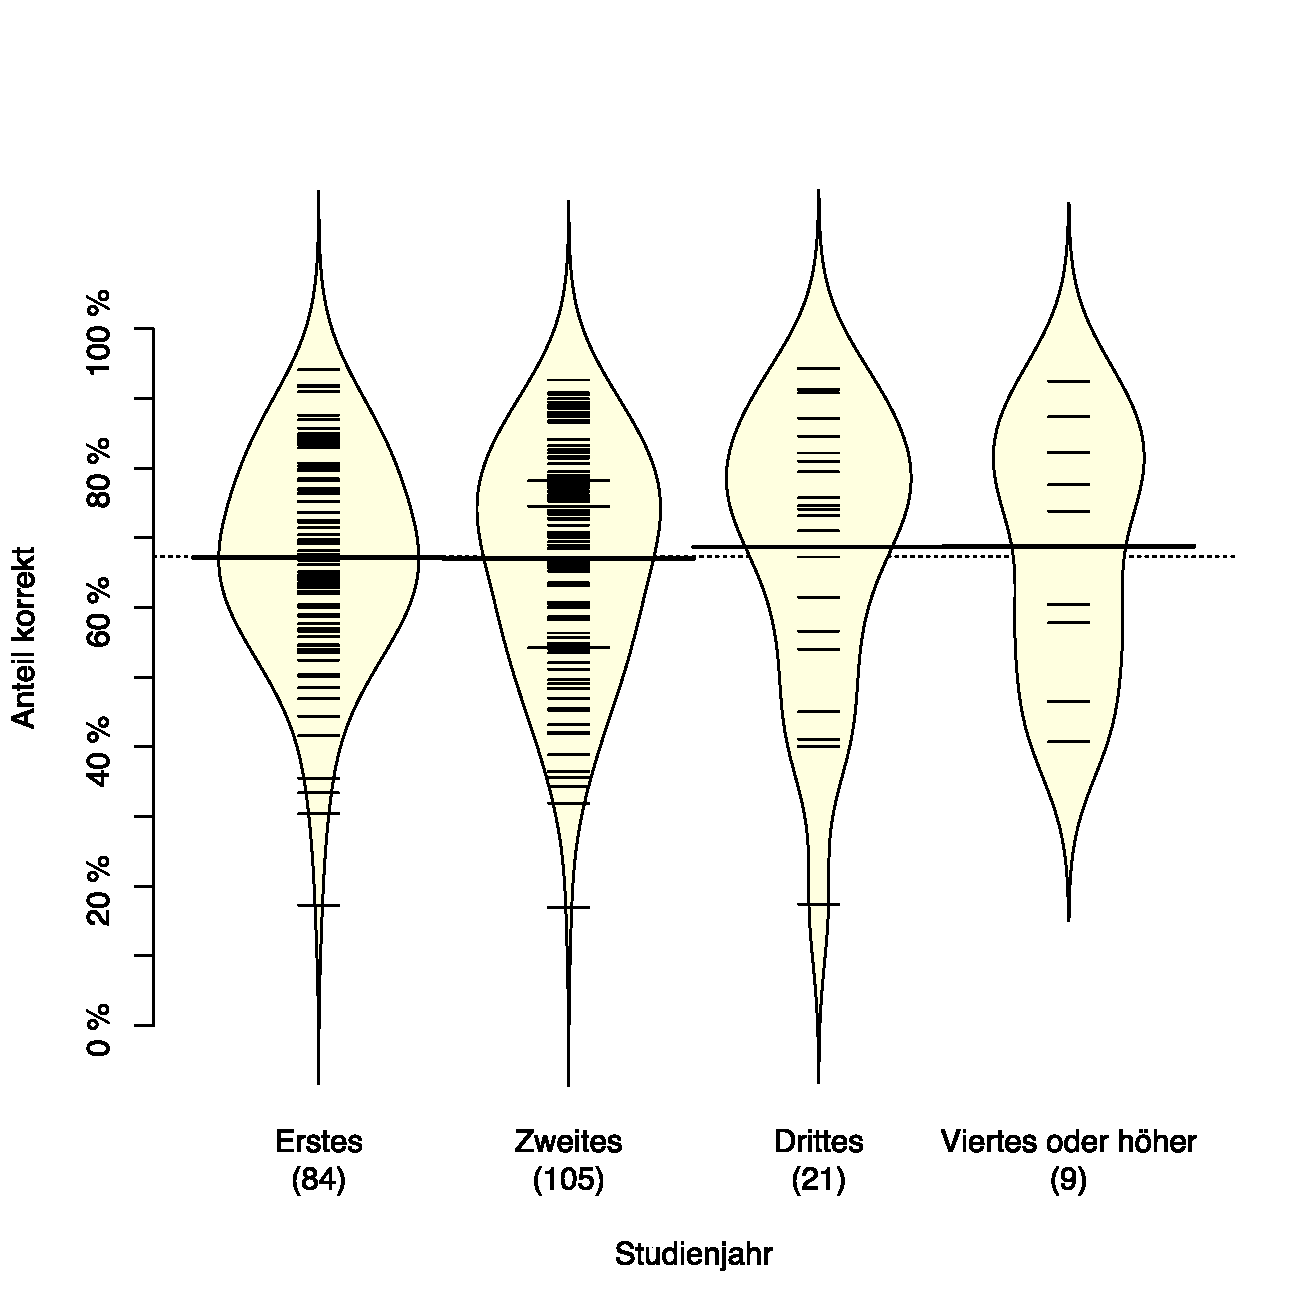
\includegraphics{figures/semester}}
  \caption{Verteilung der erreichten Prozent im Experiment aus \citet{SchaeferSayatz2017a}, gegliedert nach Studienjahr in einem sogenannten Beanplot; jede kurze waagerechte Linie entspricht einem individuellen Ergebnis, die Hüllen entsprechen einer Dichteschätzung der empirischen Verteilung pro Gruppe, die dicken längeren waagerechten Linien markieren den Mittelwert pro Gruppe}
  \label{fig:grammatikkentnissevonstudierenden002}
\end{figure}

Wie man leicht sieht, werden die Ergebnisse im verlauf des Studiums im Mittel nicht besser.
Es gibt eine leichte Verschiebung der Verteilung (des Bauchs der jeweiligen Beanplots) nach oben, insbesondere im dritten Studienjahr.
Allerdings wäre schon aufgrund des Ausscheidens leistungs- und motivationsschwächerer Studierender (Fachwechsel oder Studienabbruch) im Laufe der Semester eine stärkere Verbesserung der Leistung zu erwarten.
Wie wir in \citet[242--243]{SchaeferSayatz2017a} argumentieren, kann der Grund der beobachteten Stagnation nicht lokal in der Freien Universität gesucht werden, da sich im Vergleich der Kurrikula mehrerer Universitäten aus verschiedenen Bundesländern zeigt, dass die Freie Universität ein sehr typisches Profil in ihren germanistischen Studiengängen anbietet.

Wir gehen davon aus, dass das Problem vielmehr eine meist nicht optimale Kopplung der universitären Inhalte an die Berufsziele der Studierenden ist.
Wie oben deutlich wurde, sind ca.\ 75\% der Studierenden an der Freien Universität angehende Lehrpersonen, und die Lehre müsste sich deutlich an diesem Berufsziel orientieren.
Von einer anderen Seite nähern sich auch \citet{TopalovicDuenschede2014} demselben Problem.
In einer Bundesweiten Umfrage mit 1.019 Lehrpersonen aus allen Schulformen fanden Sie im Jahr 2013 heraus, dass 48\% der Lehrpersonen sich durch ihre Ausbildung nicht hinreichend auf den Grammatikunterricht vorbereitet fühlen \citep[76--77]{TopalovicDuenschede2014}.


\subsection{Studentische Sichtweisen auf Studium und Schulunterricht}
\label{sec:studentischesichtweisenaufstudiumundschulunterricht}

\begin{figure}[htpb]
  \centering
  \resizebox{0.9\textwidth}{!}{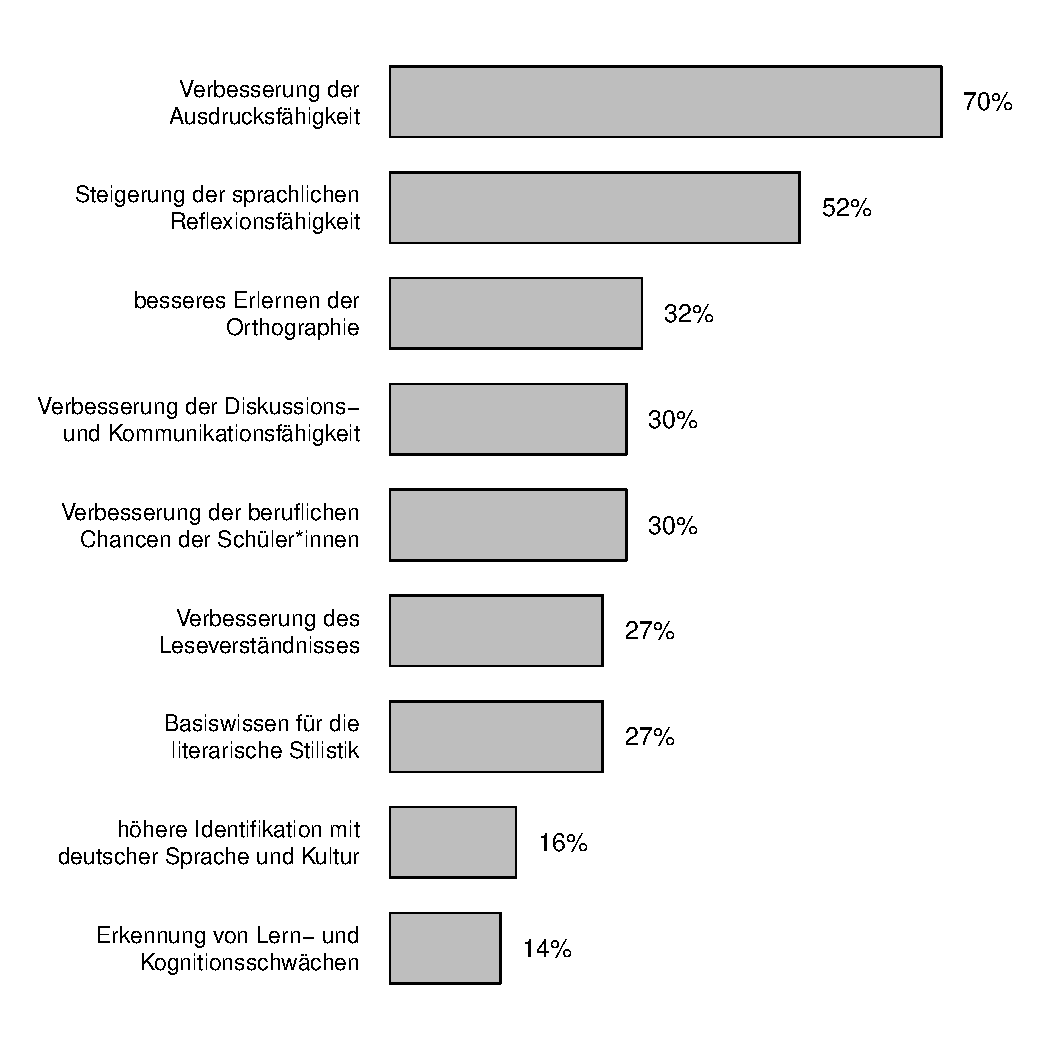
\includegraphics{figures/funktionengrammatikunterricht}}
  \caption{}
  \label{fig:studentischesichtweisenaufstudiumundschulunterricht001}
\end{figure}






\section{Form und Funktion in der Grammatik}
\label{sec:formundfunktionindergrammatik}

Zunächst ist festzustellen, dass frühere Auflagen dieses Buches aufgrund bestimmter Formulierungen und Analysen teilweise missverstanden wurden, und dass dieses Missverständnis direkt die Tauglichkeit des Buches für das Lehramtsstudium berührt.
Ein anonymes Gutachten der ersten Auflage attestierte dem Buch (recht kritisch) einen radikal formalistischen Ansatz, der grammatische Mittel vollständig losgelöst von ihrer Funktion betrachtet, und der damit das Wesentliche der Sprache, also ihre bedeutungsvermittelnden und kommunikativen Funktionen außer acht lässt.
So radikal klangen zugegebenermaßen auch einige Formulierungen in den einleitenden Kapiteln des Buches, die bis zur dritten Auflage erheblich abgetönt, aber bewusst nicht vollständig entfernt wurden.
Für die schulische Lehre wäre solch ein radikaler Ansatz jedoch völlig verfehlt und geradezu anachronistisch, und auch in der universitären Lehre wäre ein rein formorientierter Ansatz hochgradig fragwürdig.%
\footnote{Das Adjektiv \textit{anachronistisch} ist hier auf Basis der Geschichte des schulischen Unterrichts in deutscher Grammatik zu verstehen, die \zB in den Abschnitten~3.1 und~3.2 aus \citet{Bredel2013} zusammengefasst wird.}
Das Buch versteht sich aber einerseits nicht als exklusive Lektüre für das gesamte Studium.
Es sollte also von weiterer Lektüre flankiert werden, die dann das gesamte relevante Spektrum der Linguistik des Deutschen abdeckt.
<++>

Außerdem bewies dieser Text trotz einer stellenweise formlastigen Rhetorik von der ersten Auflage an, dass es die Beziehung von Form und Funktion durchaus berücksichtigt, zum Beispiel bei der Beschreibung der Intonation (Kapitel~\ref{sec:phonologie}), der Flexionskategorien (Kapitel~\ref{sec:nominalflexion} und ~\ref{sec:verbalflexion}) oder bei der Behandlung von semantischen Rollen und Passivphänomenen (Kapitel~\ref{sec:relationenundpraedikate}).

Es muss hier jedoch vor allem zwischen \textit{systeminterner} und \textit{systemexterner} (\zB kommunikativer) Funktion unterschieden werden.\index{Form und Funktion}
Das System der vier nominalen Kasus ist zum Beispiel nur äußerst schlecht mit \textit{systemexternen} Funktionen zu verbinden, die direkt irgendetwas mit Semantik, Pragmatik, Textaufbau und Argumentationstechniken etc.\ zu tun haben.
Seine \textit{systeminterne} Funktion im grammatischen System ist allerdings von erheblicher Wichtigkeit, insbesondere angesichts der Möglichkeiten des Deutschen, die Bestandteile von Sätzen vergleichsweise frei im Satz zu positionieren.
Der Kasus eines Nomens kodiert nämlich vor allem die Relation dieses Nomens zu einem Verb (und im Fall des Genitivs primär zu einem anderen Nomen), und zwar in starker Abhängigkeit von teilweise auch semantisch motivierbaren Typen von Verben.%
\footnote{Ein Feuerwerk der systeminternen funktionalen Betrachtung ergibt sich in diesem Zusammenhang durch das Einbeziehen der Kasussynkretismen, also des Zusammenfalls von Formen.
Dieser fällt je nach Genus, Flexionsklasse und Numerus ganz unterschiedlich aus.
Zudem müssen Substantive, Adjektive und Artikel insgesamt betrachtet werden, da sie auf unterschiedliche Weise an der Kasusmarkierung beteiligt sind und einander diese sogar gegebenenfalls abnehmen.
Kapitel~\ref{sec:nominalflexion} beschäftigt sich ausführlich mit dem Kasussystem.}
Während also Kasus nicht direkt semantisch interpretierbar ist, ist er dennoch von großer Bedeutung für die Konstruktion der Bedeutung von Sätzen.
Darauf wird in dieser Einführung bei zahlreichen Gelegenheiten vertiefend eingegangen.
Wir geben Definition~\ref{def:internexternefunktion}, die sich auf Konzepte rückbezieht, die in Kapitel~\ref{sec:grammatik} eingeführt wurden.
Kapitel~\ref{sec:grundbegriffedergrammatik} führte bereits vertiefend in systeminterne Funktionen ein, zum Beispiel mit Begriffen wie \textit{Merkmal} und \textit{Wert} oder \textit{Relationen} (\textit{Strukturbildung}, \textit{Rektion} und \textit{Kongruenz}).

\Definition{Systeminterne und systemexterne Funktion}{\label{def:internexternefunktion}%
Sprachliche Formen (Formen von Wörtern, Sätzen usw.) haben durch die überwiegende Regelmäßigkeit ihrer Bildungen und Kombinationsmöglichkeiten eine Systematik (die Grammatik).
Systeminterne Funktionen grammatischer Mittel sind solche, die innerhalb dieses Systems gelten, \zB die Funktion von Kasus bei der Markierung von Beziehungen zwischen Nomina und Verben.
Systemexterne Funktionen grammatischer Mittel sind ihre Bedeutungen, ihre systematischen Beiträge zur Konstruktion von Kommunikationssituationen und Texten, ihre Art, bestimmte Register und Stile zu markieren usw.
\index{Funktion!systemintern und systemintern}
}

Es ist nun nicht davon auszugehen, dass sich interne und externe Funktionen stets sauber voneinander trennen lassen, und eine umfassende Betrachtung ist sicherlich das Ziel der Grammatikforschung und des Studiums.
Die Motivation, diese Einführung dennoch stark (wenn auch nicht dogmatisch) an der Form sprachlicher Äußerungen und ihren systeminternen Funktionen auszurichten, begründet sich aus meiner persönlichen Lehrerfahrung im Fach Deutsche Philologie.
Während diese Erfahrung gewiss subjektiven und anekdotischen Charakter hat, wurde sie durch \citet{SchaeferSayatz2017a} auf methodisch stringente Weise bestätigt, worauf in Abschnitt~\ref{sec:grammatikkentnissevonstudierenden} ausführlicher eingegangen wird.
Programmatisch formuliert setzt die \textit{systematische} Betrachtung von Form und Funktion sprachlicher Einheiten -- um die es nach meiner Auffassung sowohl in der Schule bzw.\ Fachdidaktik als auch in der universitären Ausbildung bzw.\ Fachwissenschaft geht -- eine genaue Kenntnis der Systematik der Formen und ihrer systeminternen Funktionen voraus.%
\footnote{Abweichende Versuche der Didaktik früherer Jahrzehnte bestätigen wahrscheinlich dieses Programm indirekt eher als dass sie es widerlegen, siehe Abschnitt~\ref{sec:deutschunterrichtunddiewellenderdidaktik} und die dort zitierte Literatur.}
In der universitären Lehre aber davon auszugehen \textit{oder zu verlangen}, dass Studierende vor dem ersten Semester bereits eine ausreichende Kenntnis des formalen grammatischen Systems erworben haben, ist allerdings verfehlt und potentiell fatal für ihre Ausbildung und ihre spätere berufliche Praxis.
Auch wenn es vielleicht nicht immer eine Mehrheit der Studierenden betrifft, so wird doch in der frühen Phase des Studiums immer wieder gerne Kasus direkt mit Bedeutungen identifiziert und mit den unzureichenden \textit{Grammatikerfragen} ("`\textit{wer oder was}"' usw.) analysiert (s.\ Abschnitt~\ref{sec:kasus}), grammatisches Genus wird mit Bedeutungsklassen identifiziert, Subjekte werden als der "`Satzgegenstand"' \textit{definiert}, aber mit dem Nominativ \textit{identifiziert}, Wortarten werden semantisch motiviert usw.%
\footnote{Gleichermaßen werden nahezu rein formale Phänomene nicht zuverlässig beschrieben.
Dass zum Beispiel die \textit{Klatschmethode} (s.\ Abschnitt~\ref{sec:silben}) bei der Beschreibung der Silbentrennung nicht besonders weit trägt, ist Studierenden meist bewusst.
Die Fähigkeit, die Silbifizierung im Deutschen und ihre graphematischen Folgen anderweitig und präzise zu beschreiben, kann und darf hingegen trotzdem nicht vorausgesetzt werden.}
Während alle diese Phänomene (einschließlich der Wortklassen) hochinteressante und relevante Beziehungen zur Bedeutung sowie zahlreiche andere externe Funktionen haben, haben sie doch zunächst eine formale Seite und Systematik, die für jede weitere Betrachtung bekannt sein muss.
Die insgesamt stark formorientierte Ausrichtung des Buches entspringt also der Überzeugung, dass vor allen funktionalen Betrachtungen, die selbstverständlich Teil des Studiums sein sollten, mit einer gründlichen Analyse der Form und der systeminternen Funktionen begonnen werden sollte, die auch mit eingebrannten bedeutungsfixierten Didaktisierungen aus der Schulzeit (wie den semantischen Definitionen von Wortklassen) aufräumt.

Komplexere Phänomene wie -- um ein arbiträres Beispiel herzunehmen -- Relativsätze werden zudem von Studierenden zu Studienbeginn formal oft gar nicht verstanden, und eine Diskussion über ihre Funktion erübrigt sich damit.
Sehen wir uns die Folgen einer unzureichenden formalen Analyse etwas genauer an.
Es ist gewiss ein vordergründig rein formaler Sachverhalt, dass ein Relativsatz ein im Prinzip vollständiger Satz ist, der aber so konstruiert wird, dass eins der in ihm vorkommenden "`Satzglieder"' (besser gesagt eine der Ergänzungen und Angaben, s.\ Abschnitte~\ref{sec:valenz} und~\ref{sec:konstituentenundsatzglieder}) durch ein spezielles Pronomen realisiert wird, welches sich dann auf ein Bezugsnomen außerhalb des Relativsatzes bezieht.
Das Bezugsnomen steuert die semantische Interpretation (Bedeutung) des Relativpronomens bei.
Wir erhalten (\ref{ex:formundfunktionindergrammatik002}) parallel zu (\ref{ex:formundfunktionindergrammatik001}) als einen einfachen Fall eines Relativsatzes.

\begin{exe}
  \ex
  \begin{xlist}
    \ex{\label{ex:formundfunktionindergrammatik001} Eine\slash die Kommilitonin hat gelacht.}
    \ex{\label{ex:formundfunktionindergrammatik002} eine\slash die Kommilitonin, die gelacht hat}
  \end{xlist}
\end{exe}

Es fällt rein formal auf, dass zumindest die Verbformen im Relativsatz andere Positionen einnehmen als im unabhängigen Satz.
Dass (und \textit{auf welche Weise}) dies völlig regelmäßig geschieht, muss allerdings erst einmal verstanden werden, um die Beziehung zwischen den beiden Konstruktionen überhaupt wahrnehmen zu können.
Wird das durch einen Relativsatz modifizierte Substantiv wie in (\ref{ex:formundfunktionindergrammatik003}) in einer übergeordneten Satzperiode verwendet, wird die systeminterne Funktion schnell klar.
Der Relativsatz ermöglicht es uns stark vereinfacht gesagt, zwei im Grunde vollständige Sätze zu einem zu kombinieren (Hypotaxe).
Im Gegensatz zu einer einfachen aufzählenden Verbindung (Parataxe) wie in (\ref{ex:formundfunktionindergrammatik004}) nutzt der Relativsatz die Identität eines nominalen Bezugs (also der Bedeutung zweier Nomina) und vermeidet dadurch die zweimalige unabhängige Aufnahme der semantischen Referenz.

\begin{exe}
\ex
\begin{xlist}
  \ex{\label{ex:formundfunktionindergrammatik003} Die Kommilitonin, die gelacht hat, heißt Camilla.}
  \ex{\label{ex:formundfunktionindergrammatik004} Eine Kommilitonin hat gelacht, und die\slash sie heißt Camilla.}
\end{xlist}
\end{exe}

Die systeminterne Funktion hat also eine semantische Funktion in ihrem Gefolge, die in ihrer Systematik nur als Folge der formalen zu verstehen ist.
Die Erkenntnis, dass darüberhinaus die ebenfalls externe \textit{textuelle} oder \textit{rhetorische Funktion} eines Relativsatzes in den Bereichen des \textit{Verdichtens} und \textit{Präzisierens} anzusiedeln ist, kann nur in Zusammenhang mit den ersten beiden Schritten vollzogen werden.
Ohne diese Schritte kann überhaupt nicht sicher identifiziert werden, was ein Relativsatz denn überhaupt sein soll, woran wir ihn erkennen und wie wir ihn formulieren.
Selbst wenn wir davon ausgehen, dass (\ref{ex:formundfunktionindergrammatik003}) und (\ref{ex:formundfunktionindergrammatik004}) bedeutungsgleich (aber eventuell rhetorisch verschieden) sind, kommen wir nicht umhin, festzustellen, dass ihre Verwendung hochgradig stil-, register- und medienspezifisch ist, womit weitere externe Funktionen angesprochen werden.
In fast allen bildungs- und schriftsprachlichen Kontexten ist nämlich davon auszugehen, dass (\ref{ex:formundfunktionindergrammatik004}) unangenehm auffällt.
Verdichtungen und Präzisierungen, die komplexere formale Mittel wie Relativsätze einsetzen, kennzeichnen nämlich genau solche Kontexte, und wir irritieren unser sprachliches Gegenüber im Ernstfall erheblich, wenn wir in der Bildungssprache zu ausufernder Parataxe greifen.

Ganz unabhängig davon sehen wir an (\ref{ex:formundfunktionindergrammatik004}), dass die systeminternen Interaktionen weiter reichen, als uns vielleicht lieb ist.
Die parataktische Version zwingt uns nämlich, zweimal einen Artikel bzw.\ ein Pronomen zu verwenden.
Hier wurde zuerst der indefinite \textit{eine} und dann das Definitpronomen \textit{die} oder alternativ das Personalpronomen \textit{sie} verwendet.
Die andere mögliche Variante wäre die in (\ref{ex:formundfunktionindergrammatik005}), wobei diese sich allerdings bereits im Grenzbereich zwischen stilistischem Mangel und Ungrammatikalität bewegt.

\begin{exe}
  \ex[?]{\label{ex:formundfunktionindergrammatik005} Die Kommilitonin hat gelacht, und die\slash sie heißt Camilla.}
\end{exe}

Gehen wir noch weiter und sehen uns informationsstrukturelle Funktionen an, stellen sich auch diese als mit der Form eng verknüpft heraus.
Weder (\ref{ex:formundfunktionindergrammatik004}) noch (\ref{ex:formundfunktionindergrammatik005}) sind nämlich wirklich robust bedeutungsgleich mit (\ref{ex:formundfunktionindergrammatik003}).
Ohne tief in die Details zu gehen, zeigt (\ref{ex:formundfunktionindergrammatik007}) durch eine besondere Betonung (also ein formales Mittel), dass wir dank des Relativsatzes Ausdrucksmöglichkeiten haben, die wir mit der parataktischen Version schlichtweg nicht haben.
Die in Majuskeln geschriebenen Silben sind mit hervorhebender Betonung zu lesen.

\begin{exe}
  \ex{\label{ex:formundfunktionindergrammatik007} DIE Kommilitonin, die geLACHT hat, heißt Camilla.}
\end{exe}

In geschriebenen Texten markieren wir Intonation normalerweise nicht.
Dort werden die entsprechenden Sätze ohne besondere Markierungen aber trotzdem ähnlich verwendet, oder es kommen andere Markierung wie zum Beispiel Adverbiale oder besondere Wortstellungen zum Zug.
Als Beispiel wird in (\ref{ex:formundfunktionindergrammatik008}) ein Aufzählungskontext gegeben.
Ohne Relativsätze wären wir hier im Ausdruck erheblich eingeschränkt.

\begin{exe}
  \ex{\label{ex:formundfunktionindergrammatik008} Die etwas ruhigere Kommilitonin heißt Kiki. Die Kommilitonin (hingegen), die gelacht hat, heißt Camilla.}
\end{exe}

Gleichermaßen gibt es für Sätze wie (\ref{ex:formundfunktionindergrammatik009}), die allgemeine Aussagen formulieren, kaum eine semantisch adäquate parataktische Variante, die eine vertretbare Länge hat und stilistisch unauffällig ist.

\begin{exe}
  \ex{\label{ex:formundfunktionindergrammatik009} Die Mitspielerin, die zuletzt lacht, gewinnt.}
\end{exe}

Wir feiern mit dem Relativsatz also ohne weiteres ein grammatisches Fest, bei dem Wissen aus unterschiedlichsten Teilen der Grammatik abgerufen wird.
Um die semantischen, textuellen und rhetorischen, stilistischen und registerbezogenen Funktionen von Relativsätzen zu benennen, müssen wir in der Lage sein, Relativsätze zu erkennen, ihre Form zu analysieren, und dieses Wissen in einen größeren Zusammenhang zu stellen.

Wir sind weiter oben von der Frage ausgegangen, welche Kenntnisse Studierende in die Lehramtsausbildung mitbringen, und wir haben argumentiert, dass formale Analysen eine Bedingung für eine systematische funktionale Betrachtung von Sprache sind.
Angesichts der Komplexität des grammatischen Systems und der externen Funktionen grammatischer Mittel (wie am Beispiel des Relativsatzes vorgeführt) können wir davon ausgehen, dass es zielführender ist, im Studium einen systematischen Neuanfang zu wagen, der sich nicht auf vermeintlich vorhandenes Schulwissen stützt.
Die fundamentale Rechtfertigung dieses Ansatzes liegt zudem in der oft übersehenen Tatsache, dass der Grammatikunterricht in der Schule grundlegend andere Ziele verfolgt als die universitäre Ausbildung von zukünftigen Lehrpersonen.
Darum wird es in diesem Kapitel weiter unten noch ausführlicher gehen.

Nicht kontrovers ist allerdings die Minimalforderung, dass Lehrkräfte, die von Universitäten und Hochschulen mit einem erfolgreichen Studienabschluss in das Schulfach Deutsch entlassen werden, diejenigen Kenntnisse mitbringen müssen, die sie Kindern und Jugendlichen vermitteln sollen.
Das Studium muss diese Kenntnisse über den weitaus höheren Anspruch des spezifischen Studienwissens hinaus sicherstellen.
In diesem Zusammenhang ist es nun bemerkenswert, dass Dozierende an Universitäten oft keinerlei Daten darüber haben, was sie bei Studierenden voraussetzen können und was nicht.
Hier ist dringend nachzuhelfen, vor allem weil die Gefahr besteht, dass ein in seinem oft nicht gut definiertes \textit{Schulwissen} von Lehrpersonen an Universitäten stillschweigend vorausgesetzt und auf dieses "`aufgebaut"' wird.
In diesem Zuge treten wir auch aus dem Nebel des Anekdotischen heraus und sehen empirisch klar in Abschnitt~\ref{sec:kenntnisseerwartungenundmotivationvonstudierenden}.


